\subsection{Feedback Control Systems}
\subsubsection{Review of Signal and Systems}
\begin{enumerate}
    \item Elementary Signals. \\
    Please refer basic signals in the Chapter \textbf{Signal and Systems}. \\
    Complex Exponential function $Ae^{zt}$, where $z = \sigma + j\omega$.
    \begin{align*}
        y(t) &= Ae^{(\sigma+j\omega)t} = Ae^{\sigma t}e^{j\omega t} \\
        &= Ae^{\sigma t}[\cos(\omega t) + j\sin(\omega t)] \\
        \Re\{Ae^{zt}\} &= Ae^{\sigma t}\cos(\omega t) \\
        \Im\{Ae^{zt}\} &= Ae^{\sigma t}\sin(\omega t)
    \end{align*}
    Note that that when $\sigma < 0$, the signal exponential damped.
    \item Interconnection of systems
    \begin{enumerate}
        \item cascade (or series): $\displaystyle y = G(Fu) = GFu$ \\
        \begin{center}
        \begin{tikzpicture}[auto, node distance=2cm,>=latex']
            \node [draw, rectangle] (block1) {F};
            \node [draw, rectangle, right of=block1] (block2) {G};
            \draw [->] (-1,0) -- node[name=u] {u} (block1);
            \draw [->] (block1) -- (block2);
            \draw [->] (block2) -- node[name=y] {y} (3,0);
        \end{tikzpicture}
        \end{center}
        \item sum (or parallel) : $\displaystyle y = Fu + Gu$
        \begin{center}
            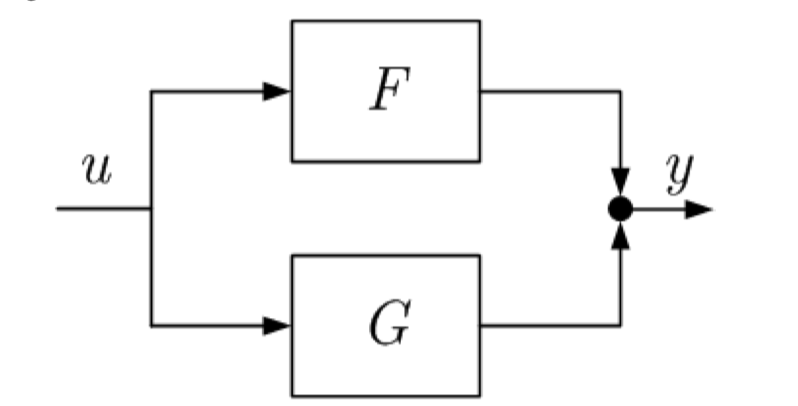
\includegraphics[width=0.5\linewidth]{image/sum.png}
        \end{center}
        \item Feedback: $\displaystyle y = F(u-Gy)$
        \begin{center}
            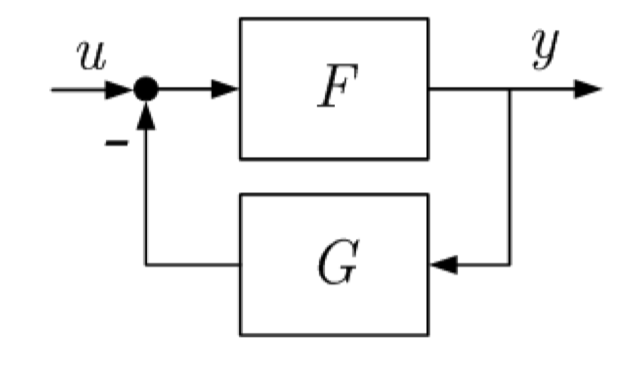
\includegraphics[width=0.45\linewidth]{image/feedback.png}
        \end{center}
    \end{enumerate}
    \item System Models
    \begin{enumerate}
        \item Electrical Circuits
        \begin{enumerate}
            \item Resistor: $\displaystyle v_R(t) = Ri_R(t)$
            \item Capacitor: $\displaystyle v_C(t) = \frac{1}{C}\int_0^{t}i_C(\tau)d\tau$  \hfill $i_C(t) = C\frac{dv_C(t)}{dt}$ \\
            LT domain: $\displaystyle V_C(s) = \frac{I(s)}{sC}$ \hfill  $\displaystyle Z_C(s) = \frac{1}{sC}$
            \item Inductor: $\displaystyle v_L(t) = L\frac{di_L(t)}{dt}$ \\
            LT domain: $\displaystyle V_L(s) = sLI(s)$ \hfill $\displaystyle Z_L(s) = sL$
        \end{enumerate}
        \item Linear Motions
        \begin{enumerate}
            \item Mass: $\displaystyle f(t) = M \frac{d^2x(t)}{dt}$
            \item Spring: $\displaystyle f(t) = Kx(t)$
            \item Damper: $\displaystyle f(t) = f_v\frac{dx(t)}{dt}$
        \end{enumerate}
        \item Angular Motions
        \begin{enumerate}
            \item Inertia: $\displaystyle T(t) = J\frac{d^2\theta(t)}{dt}$
            \item Spring: $\displaystyle T(t) = K\theta(t)$
            \item Damper: $\displaystyle T(t) = D\frac{d\theta(t)}{dt}$
        \end{enumerate}
    \end{enumerate}
    \item RC Circuit
    \begin{center}
        \begin{circuitikz} [american]
            \draw
            (0,0) to[V, v<=$v$] (0,2)
            to[R, l=$R$, i>^=$i$] (3,2)
            to[C, l=$C$, v<=$v_c$] (3,0) 
            to[closing switch](0,0);
        \end{circuitikz}
    \end{center}
    \begin{itemize}
        \item From the graph we can see the KVL yield: $\displaystyle v_R(t) + v_C(t) = v(t)$ 
        \item $\displaystyle Ri(t) + v_C(t) = v(t)$ 
        \item Since $\displaystyle v_C(t) = \frac{1}{C} \int i(\tau)d\tau$ or $\displaystyle i(t) = C\frac{dv_C(t)}{dt}$
        \item We have, $\displaystyle RC\frac{dv_C(t)}{dt} + v_C(t) = v(t)$ 
        \item Solving the first order equation, we have : 
        \item $\displaystyle v_c(t) = (v_c(0) - V)e^{-\frac{t}{RC}} + V$
    \end{itemize}
\end{enumerate}

\subsubsection{Review of Laplace Transform and Transfer Function}
\begin{enumerate}
\item  Why Laplace Transformation? \\
It converts integral and differential equations into algebraic equations.\\
\[
\begin{array}{|c|c||c|c|}
\hline
f(t) & F(s) & f(t) & F(s) \\
\hline
\delta(t) & 1 & \sin(bt) & \dfrac{b}{s^2+b^2} \\
U(t) & \dfrac{1}{s} & \cos(bt) & \dfrac{s}{s^2+b^2} \\
t & \dfrac{1}{s^2} & e^{-at} \sin(bt) & \dfrac{b}{(s+a)^2+b^2} \\
t^k & \dfrac{k!}{s^{k+1}} & e^{-at} \cos(bt) & \dfrac{s+a}{(s+a)^2+b^2} \\
e^{-at} & \dfrac{1}{s+a} & & \\
te^{-at} & \dfrac{1}{(s+a)^2} & & \\
\dfrac{1}{(k-1)!}t^{k-1}e^{-at} & \dfrac{1}{(s+a)^k} & & \\
\hline
\end{array}
\]
\item Derivative of LT \\
For higher order derivative: 
\[\displaystyle \mathscr{L}\{f^n(t)\} = s^n F(s) - \sum_{k=0}^{n-1} s^{n-1-k} f^k(0^-)\]
\item Integral of LT \\
Given $\displaystyle g(t) = \int_0^t f(\tau)d\tau$ then $\displaystyle G(s) = \frac{1}{s}F(s)$
\item Derivative of Transform Multiplication by time
\[F'(s) = \mathcal{L}\{-tf(t)\}\]
\[\frac{d^n}{ds^n}F(s) = (-1)^n \mathcal{L}\{t^n f(t)\}\]
For example : 
\[\mathcal{L}\{t\sin\omega t\} = -\frac{d}{ds} \left( \frac{\omega}{s^2 + \omega^2} \right) = \frac{2\omega s}{(s^2 + \omega^2)^2}
\]
\newpage
\item Other Properties of Laplace Transform
    \begin{table}[h]
    \begin{center}
    \begin{tabular}{|c|c|c|}
    \hline
    \textbf{Time Function} & \textbf{Laplace Transform} & \textbf{Comments} \\ \hline
    $\alpha f(t) + \beta g(t)$ & $\alpha F(s) + \beta G(s)$ &  Superposition \\ \hline
    $f(t - t_0)$ & $e^{-st_0}F(s)$ & Time delay $(t_0 \geq 0)$ \\ \hline
    $f(at)$ & $\displaystyle \frac{1}{|a|}F\left(\frac{s}{a}\right)$ & Time scaling  \\ \hline
    $e^{-at}f(t)$ & $F(s + a)$ & Shift in frequency \\ \hline
    $f^n(t)$ & $\displaystyle s^n F(s) - \sum_{k=0}^{n-1}s^{n-1-k}f^{(k)}(0^-)$ & Differentiation \\ \hline
    $\int_{0}^{t} f(\tau)d\tau$ & $\frac{1}{s}F(s)$ & Integration \\ \hline
    $f(t) * g(t)$ & $F(s)G(s)$ & Convolution \\ \hline
    $tf(t)$ & $-\frac{d}{ds}F(s)$ & Multiplication by time \\ \hline
    $f(0+)$ & $\displaystyle \lim_{s\to\infty} sF(s)$ & Initial value theorem \\ \hline
    $\displaystyle \lim_{t\to\infty} f(t)$ & $\displaystyle \lim_{s\to0} sF(s)$ & Final value theorem \\ \hline
    \end{tabular}
    \end{center}
    \caption{Laplace Transforms and their Time Functions}
    \label{table:laplace}
    \end{table}
\item Inverse Laplace Transform\\
Steps to take:
\begin{enumerate}
    \item Simplify complicated functions using partial fractions expansion.
    \item Obtain the inverse Laplace transform, $f(t)$ using the LT table.
\end{enumerate}
\item Transfer Function \\
A transfer function $G(s)$ is the ration of the Laplace transform of the output to the Laplace transform of the input.
\begin{equation}
    G(s) = \frac{Y(s)}{U(s)}
\end{equation}
Take note that we assume all initial conditions on the system are zero.
\end{enumerate}


\subsubsection{Dynamic Response}
\textbf{Common type of responses}
\begin{enumerate}
    \item Impulse response :  relate to transfer function.
    \item Step response : relate to physical parameters in LTI systems.
    \item Sinusoidal response : relate to frequency response of the system.
\end{enumerate}
\textbf{Poles and Zeros}
\begin{enumerate}
    \item System poles are the roots of the denominator polynomial of the transfer fucntion $G(s)$.
    \item The poles of the system determine its stability properties.
    \item The poles of the system determine the natural behaviour of the system.
\end{enumerate}
\textbf{Impulse responses}
\begin{enumerate}
    \item Impulse response ... \\
    Suppose the transfer function of a LTI system is
    \[G(s) = \frac{Y(s)}{U(s)}\]
    Its impulse response is given by $u(t) = \delta(t)$ and $U(s) = 1$ then, We will have $Y(s) = G(s)$. The inverse LT gives 
    \[y(t) = \mathscr{L}^{-1}\{G(s)\}=g(t) \quad G(s) = \mathscr{L}\{\text{Impulse Response}\}\]
    \item First Order System \\
    Consider a first order system $\displaystyle G(s) = \frac{1}{s+\sigma}$. Inverse Laplace transformation gives $g(t) = e^{-\sigma t}$. \\
    The time constant of the system $\tau$ is defined as $\displaystyle \tau = \frac{1}{\sigma}$ as $\displaystyle \frac{1}{e} = 0.368$ times the initial value. \\
    Note that the shape of the system response is dominated by the shape of the \textbf{smaller pole}.
    \item Second Order System \\
    A standard $2^{nd}$ order transfer function is expressed as
    \[H(s) = \frac{K \omega_n^2}{s^2 + 2 \zeta \omega_n s + \omega_n^2} = \frac{K \omega_n}{(s + \zeta \omega_n)^2 + \omega_n^2 (1 - \zeta^2)}\]
    The impulse response is given by
    \[y_i(t) = h(t) = \frac{K \omega_n}{\sqrt{1 - \zeta^2}} e^{-\sigma t} \sin(\omega_d t)\]
    The step response is given by
    \[y_s(t) = K - \frac{K}{\sqrt{1 - \zeta^2}} e^{-\sigma t} \sin(\omega_d t + \cos^{-1}(\zeta))\]
    \item Poles position and impulse responses
    \begin{itemize}
        \item real, positive poles correspond to growing exponential terms
        \item real, negative poles correspond to decaying exponential terms
        \item a poles at $s = 0$ correspond to a constant term
        \item complex pole pairs with positive real part correspond to exponentially growing sinusoidal terms
        \item complex pole pairs with negative real part correspond to exponentially decaying sinusoidal terms
        \item pure imaginary pole pairs correspond to sinusoidal terms
        \item repeated poles yield same types of terms, multiply by powers of t
    \end{itemize}
\end{enumerate}
\textbf{Step responses}
\begin{enumerate}
    \item For a step response $\displaystyle Y_s(s) = G(s)U(s)$, $\displaystyle y_s(t) = \mathscr{L}^{-1} \left\{ \frac{G(s)}{s} \right\}$
    \item DC Gain \\
    This is the ratio of the output of a system to its input (presumed constant) after all transients have decayed. \\
    If the magnitude of a step input is $A$. We then have the \textit{Final Value Theorem} and the DC gain is
     \[K = \frac{\displaystyle \lim_{ t \to \infty} y(t)}{\displaystyle \lim_{t \to \infty} U(t)} = \frac{AG(0)}{A} = G(0)\]
    \item Integrator 
    \[y(t) = \int_{0}^{t} K_i u(\tau) d\tau\]
    where $K_i$ is known as the integration gain.\\
    The transfer function is 
    \[G(s) = \frac{Y(s)}{U(s)} = \frac{K_i}{s}\]
    The step response is 
    \[y(t) = K_i t\]
    Integrator is marginally stable as its impulse response is non-decreasing. 
    \item Differentiator 
    \[y(t) = K_d \frac{du(t)}{dt}\]
    where $K_d$ is the derivative gain. \\
    The transfer function is 
    \[G(s) = \frac{Y(s)}{U(s)} = K_ds\]
    The step response is 
    \[y(t) = K_d \delta(t)\]
    \item Transportation delay \\
    A type of time delay occurs in systems which require a finite time to move material or transmit signal from one point to another.
    \[y(t) = u(t-t_d), \quad t_d = \frac{\text{distance}}{\text{speed}}\]
    The transfer function is 
    \[G(s) = \frac{Y(s)}{U(s)} = e^{-st_d}\]
    \item First Order System \\
    The General transfer function is given by
    \[G(s) = \frac{Y(s)}{U(s)} = \frac{K}{\tau s+1}; \quad y(0)= 0\]
    where the pole is located at $\displaystyle s =- \frac{1}{\tau}$ \\
    The unit step response is given by
    \[y_s(t) = K - Ke^{-\frac{t}{\tau}}\]
    Steady-state output $= \lim_{s\rightarrow0}G(s) \times $magnitude of step.
    The time constant $\tau$ for step response is $63.2\%$ of the final value $K$. The $2\%$ settling time is $4\tau$ around $98\%$ of $K$.
    \item Second Order System
    The general transfer function is given by
    \[G(s) = \frac{Y(s)}{U(s)} = \frac{K \omega_n^2}{s^2 + 2 \zeta \omega_n s + \omega_n^2}; \quad y(0)=y'(0)=0\]
    Poles of a second order system $\displaystyle s = -\zeta \omega_n \pm \omega_n \sqrt{\zeta^2 -1}$
    \begin{itemize}
        \item $\zeta > 1$, poles are real and distinct, system is overdamped
        \item $\zeta = 1$, poles are real and equal (repeated), system is critically damped
        \item $\zeta < 1$, poles are complex conjugate, system is underdamped
    \end{itemize}
    A pair of complex poles can be defined in real and imaginary parts: $s = -\sigma \pm j\omega_d$. \\
    where $\sigma = \zeta \omega_n$ and $\omega_d = \omega_n \sqrt{1-\zeta^2}$ \\
    The step response of a second order system is given by
    \[y(t) = K \left( 1 - \frac{e^{-\sigma t}}{\sqrt{1 - \zeta^2}} \sin(\omega_d t + \phi) \right)\]
    The magnitude of real part of the pole, determine the exponential envelope. The farther to the left of the imaginary axis, the faster it will reach the steady state.\\
    The imaginary part of pole determine the frequency of the sinusoidal signal. The bigger the value of $\omega_d$, more oscillation will occur.\\
    For over and critically damped system, the behave more like first order systems. \\
    Effect of an additional zero on the system. This will lead to a huge hump in the early part of the step response function.    
\end{enumerate}
\textbf{Time domain specifications}
\begin{enumerate}
    \item Rise time, $t_r$ : the 10\% to 90\% rise time.
    \begin{equation}
        t_r \approx \frac{1.8}{\omega_n}
    \end{equation}
    \item Overshoot $M_p$ \\
    The overshoot formula is given by
    \begin{equation}
        M_p = Ke^{-\frac{\pi \zeta}{\sqrt{1-\zeta^2}}}, \quad 0\leq\zeta<1
    \end{equation}
    The percentage overshoot is given as
    \begin{equation}
        \%M_p = \frac{M_p}{y_{ss}}\times 100\% = e^{-\frac{\pi \zeta}{\sqrt{1-\zeta^2}}}\times 100\%
    \end{equation}
    \item Peak time $t_p$ : time it takes the system to reach the maximum overshoot point\\
    The peak time is given by
    \begin{equation}
        t_p = \frac{\pi}{\omega_d}
    \end{equation}
    \item Settling time $t_s$ : the time it takes the system transient to decay\\
    Measure of smallness: 1\%, 2\%, or 5\% have been used.
    \begin{equation}
        t_s = \frac{-\ln{(\text{Measure of smallness})}}{\zeta \omega_n} = \frac{4}{\sigma}
    \end{equation}
    
    \item Design Synthesis \\
    You should find $\omega_n,\;\sin^{-1}\zeta,\;\sigma$ and plot on your $s$-plane.
\end{enumerate}

\subsubsection{Feedback Control}





    